\chapter{Обзор технологий} \label{ch2}
	
Как уже было сказано в \ref{ch1:sec2} в системе будет два приложения: клиентское и серверное. Поэтому данная глава тоже будет разделена на два пункта: технологии для разработки клиентского приложения и для серверного. 

\section{Обзор технологий разработки серверных приложений]} \label{ch2:sec1}

\subsection{Выбор языка программирования} \label{ch2:subsec11}

Прежде чем приступить к рассмотрению технологий, необходимо определиться с языком программирования. Так как почти для каждого языка программирования есть библиотеки или фреймворки, поэтому при выборе языка необходимо я решил основываться на следующих критериях:

\begin{itemize}
	\item Популярность. Если у языка крупное сообщество программистов, то для него написано большое количество библиотек, а также будет проще найти ответ на форуме на возникающие вопросы, например при возникновении ошибки.
	\item Строгая/статическая типизация. У языков со строгой типизацией на этапе компиляции происходит проверка типов, и поэтому это позволяет избежать множества ошибок, связанных с типизацией, а так же ускоряет разработку.  
	\item Простота. Так же сильно ускоряет обучение и разработку приложения.
\end{itemize}  

Основываясь на один из самых известных рейтингов языков программирования \textit{«TIOBE Index»}\cite{tiobe} можно выделить 5 самых популярных языков: Python, C, Java, C++, C\#. Из данного списка под упомянутые ранее критерии подходят два языка: Java и C\#. Ввиду того, что с языком \textbf{Java} я знаком уже более 4 лет, мой выбор пал на него.

\subsection{Выбор основного фреймворка} \label{ch2:subsec12}

Определившись с языком программирования, можно перейти к выбору основной технологии. В мире Java самым популярным фреймворком является уже более 10 лет \textbf{Spring}\cite{spring}. Основные преимущества данной технологии:

\begin{itemize}
	\item Популярность. Данной технологии доверяют множество компаний по всему миру, например Яндекс или Сбербанк.
	\item Гибкость. Гибкий и всеобъемлющий набор расширений и сторонних библиотек Spring позволяет разработчикам создавать практически любые приложения, которые только можно вообразить.   
	\item Большая экосистема. Сам по себе Spring содержит только базовые функции. Остальные вы можете подключить найдя соответствующею библиотеку, например для работы с базой данных или управлением безопасностью. Из этого следует то, что вы можете подключить только то, что вам действительно необходимо.
\end{itemize}  

Основой Spring являются две принципа: Inversion of Control (IoC) and Dependency Injection (DI).

\textbf{Inversion of Control (IoC)} - это принцип состоит в том что большую часть объектов создаем не мы, а Spring. Мы лишь конфигурируем классы (с помощью аннотаций либо в конфигурационном XML), чтобы «объяснить» фреймворку Spring, какие именно объекты он должен создать за нас, и полями каких объектов их сделать. Spring управляет созданием объектов и потому его контейнер называется IoC-контейнер. А объекты, которые создаются контейнером и находятся под его управлением, называются бинами. Иллюстрация данного принципа представлена на \firef{fig:ioc}.

\begin{figure}[ht!] 
	\center
	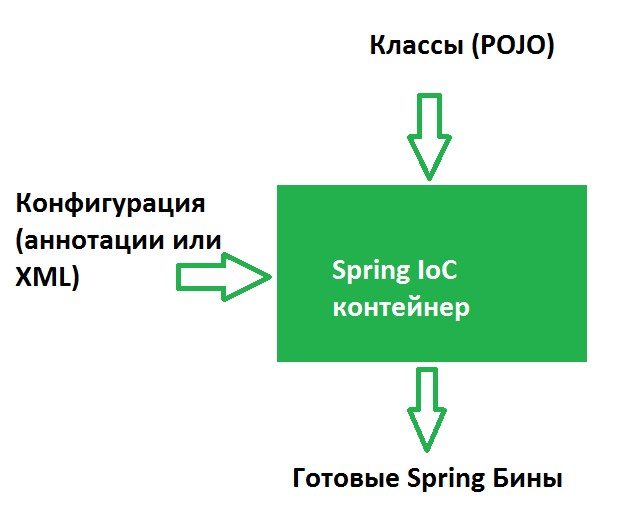
\includegraphics [scale=0.5] {my_folder/images//ioc}
	\caption{Схема Inversion of Control} 
	\label{fig:ioc}  
\end{figure}

\textbf{Dependency Injection (DI)} -  процесс предоставления внешней зависимости программному компоненту. Это означает что объект не сам создает другие объекты, необходимые для его работы, а получает их снаружи, например через конструктор класса.

На основе этих двух принципов и построена вся экосистема библиотек фреймворка. 

\subsection{Выбор дополнительных библиотек} \label{ch2:subsec13}

Как было сказано выше, фреймворк Spring позволяет подключить множество библиотек, поэтому необходимо было определиться с библиотеками, которые будут подключены дополнительно. Исходя из задания, можно было определить следующие библиотеки:

\begin{itemize}
	\item Для упрощения конфигурации и запуска приложения - Spring Boot.
	\item Для обработки входящих запросов - Spring Web.
	\item Для работы с базой данных - Spring Data Jpa. (а также flyway для применения миграции баз данных)
	\item Для работы с безопасностью (ограничение доступа) - Spring Security. (а io.jsonwebtoken.jwt для формирования JWT токенов).
	\item Для автогенерации спецификации OpenAPI - SpringDoc.
\end{itemize}  

Рассмотрим основные.

\textbf{Spring Boot} - это проект, целью которого является упрощение создания приложений на основе Spring. Он позволяет наиболее простым способом создать web-приложение, требуя от разработчиков минимум усилий по его настройке и написанию кода. Основными его преимуществами являются: простота управления зависимостями (существуют специальные starter библиотеки для более простой интеграции с Spring Boot) и автоматическая конфигурация (конфигурация всего приложения находится в специальном файле: /resources/application.yml, где описываются все необходимые параметры, например подключение к базе данных).

\textbf{Spring Web} - это библиотека из экосистемы Spring, которая добавляет все необходимое для обработки входящих HTTP запросов. Для этого в библиотеке есть специальные аннотации. На \firef{fig:spring-web-route} представлен пример метода, обрабатывающего GET запрос. 

\begin{figure}[ht!] 
	\center
	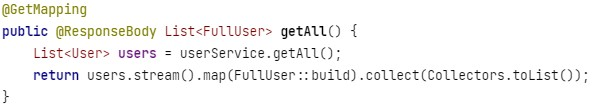
\includegraphics [scale=0.8] {my_folder/images//spring-web-route}
	\caption{Пример обработчика входящего запроса} 
	\label{fig:spring-web-route}  
\end{figure}

В данном примере наша функция принимает входящий запрос, выполняет какую-то бизнес логику, и отдает определенные модели. Остальную работу делает за нас Spring: он настраивает сервер, чтобы после приема запроса он отдавался нужной функции, самостоятельно превращает модели полученные из функции в JSON объекты и формирует ответ клиенту. 

Также библиотека позволяет проверять заголовки запроса, получать тело, настраивать динамические URL и обрабатывать их, оправлять настраиваемые коды ответов и многое другое. Все это описано в официальной документации\cite{spring}. 

\textbf{Spring Data Jpa} - это библиотека предоставляющая необходимые абстракции для работы с базой данных, из состава Spring. Основной принцип этой библиотеки заключается в том, что мы таблицы базы данных представляем как обычные классы. 

Необходимые шаги:

\begin{enumerate}
	\item[1] Создаем сущность. Для этого надо создать класс (имя совпадает с именем таблицы в БД) и пометить его аннотацией \textit{\@Entity}. Поля описанные в данном классе должны совпадать с колонками в базе.
	\item[2] Наследоваться от одного из интерфейсов Spring Data, например от CrudRepository. Данный интерфейс представляет базовые методы для работы с базой (есть и другие интерфейсы). Если нет необходимого методы, запросы к сущности можно строить прямо из имени метода. Для этого используется механизм префиксов find…By, read…By, и так далее, далее от префикса метода начинает разбор остальной части.
	\item[3] Далее уже можно использовать интерфейс в бизнес логике. Spring сам создаст необходимый класс со всеми реализациями и передаст его туда, где используется интерфейс. 
\end{enumerate} 
 
\section{Обзор технологий разработки клиентских приложений} \label{ch2:sec2}
	

\subsection{Обзор основного фреймворка} \label{ch2:subsec21} 

В качестве основного фреймворка я решил выбрать \textit{Flutter}\cite{flutter}. Это технология разработанная компанией Google, позволяющая разрабатывать мультиплатформенные приложения. На данный момент она поддерживает 6 платформ: Web, Android, IOS, Windows, Linux, MacOS. Как раз из-за этой особенности Flutter и был выбран как главная технология. 

В качестве языка программирования используется Dart. Данный язык задумывался как типизированная замена JavaScript но в веб среде язык не взлетел, но Google придумали ему другое применение. 

Преимущества FLutter:
\begin{itemize}
	\item Быстрый. Код Flutter компилируется в машинный код ARM или Intel, а также в JavaScript для быстрой работы на любом устройстве.
	\item Поддерживает горячую перезагрузку. Данная возможность позволяет перекомпилировать только те участки кода, которые поменялись и не перезапускать приложение, что в десятки раз увеличивает скорость разработки.
	\item Гибкий. Flutter позволяет управлять каждым пикселем, чтобы создавать индивидуальные адаптивные дизайны. А так же он позволяет использовать особенности платформы, например работать с камерой.
	\item Open Source. Код Flutter распространяется под меткой Open Source, что означает что он полностью открытый и каждый желающий может помочь в развитии продукта.

\end{itemize}  

Весь пользовательский интерфейс во Flutter строиться из так называемых виджетов, которые составляются в дерево. Все кнопки, тексты, картинки и прочее, что видит пользователь, является виджетом. Видимые виджеты разделяются две категории: stateless и statefull.

\textbf{Stateless} виджеты, как понятно из названия, не имеют состояния. Они нужны только для отображения какой либо части пользовательского интерфейса. Из-за отсутствия состояния, эти виджеты намного легче и производительнее.

\textbf{Statefull} виджеты наоборот содержат состояние, и позволяют вызывать обновление и перересовку экрана по изменению состояния. Во время перерисовки, обновляется как сам виджет, так и все его потомки. Для изменения состояния используется метод setState().

Чтобы создать свой виджет, необходимо создать класс и унаследовать его от базового класс (либо StatelessWidget, либо StatefullWidget). Также обязательно необходимо переопределить метод build(BuildContext context) который и отвечает за отрисовку. Данный метод вызывается на каждый отрисованный кадр. На \firef{fig:flutter-widget} представлен пример простейшего виджета.

\begin{figure}[ht!] 
	\center
	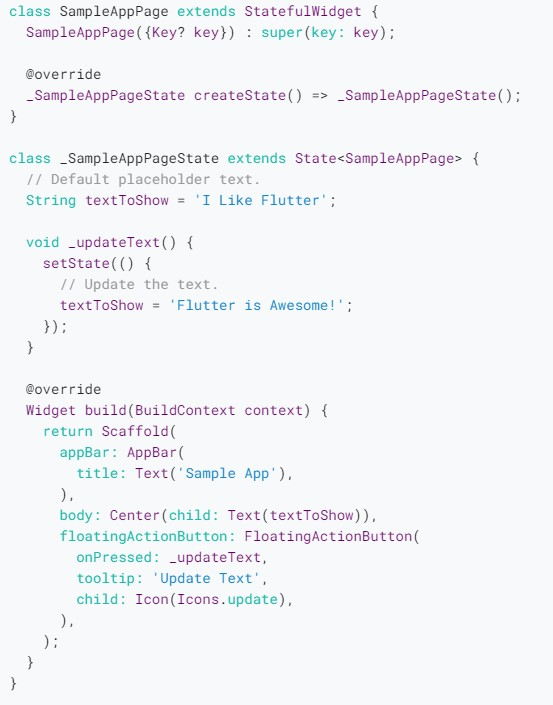
\includegraphics [scale=0.6] {my_folder/images//flutter_widget}
	\caption{Пример виджета} 
	\label{fig:flutter-widget}  
\end{figure}

В данном примере отрисовывается экран на котором представлен текст по центру и кнопка. По нажатию кнопки происходит смена текста и перерисовка экрана.

\subsection{Обзор дополнительных библиотек} \label{ch2:subsec22} 

Приложения на Flutter можно разрабатывать и без каких либо библиотек, но для удобства, гибкости и скорости разработки необходимо добавить некоторые библиотеки.

\textbf{Bloc}\cite{bloc} - это шаблон проектирования, компонент бизнес-логики, отвечающий за управление состоянием. Этот шаблон проектирования помогает отделить представление от бизнес-логики. Следование шаблону BLoC облегчает тестирование и повторное использование. Этот пакет абстрагирует реактивные аспекты шаблона, позволяя разработчикам сосредоточиться на написании бизнес-логики. На \firef{fig:bloc} представлена схема взаимодействия с блоком.

\begin{figure}[ht!] 
	\center
	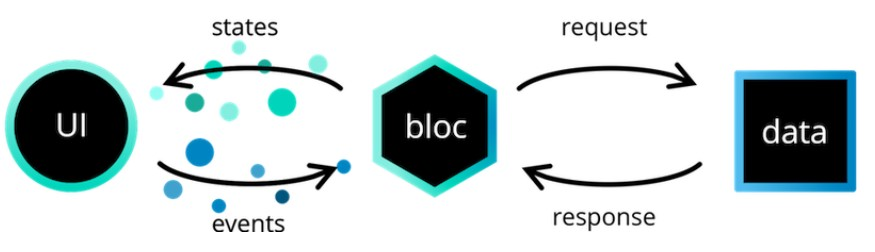
\includegraphics [scale=0.6] {my_folder/images//bloc_pattern}
	\caption{Bloc} 
	\label{fig:bloc}  
\end{figure}

Основная концепция данного шаблона в том, что создается класс у которого есть два потока: событий и состояний. После определенного действия (например пользователь нажал на кнопку) в блок добавляется новые событие, и блок начинает его обработку. Обработкой события и является бизнес логика. После необходимых действий, блок выдает наружу через соответствующий поток новое состояние которое отображает виджет. Пример простейшего блока представлен на \firef{fig:bloc-example}.

\begin{figure}[ht!] 
	\center
	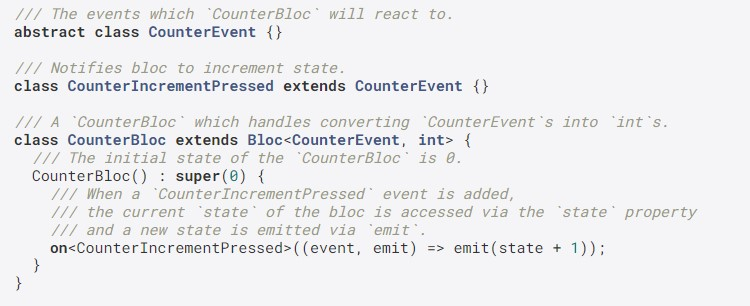
\includegraphics [scale=0.6] {my_folder/images//bloc_example}
	\caption{Пример Bloc} 
	\label{fig:bloc-example}  
\end{figure}

Так же в библиотеке поставляются специальные виджеты, которые упрощают работу с блоком. Так например, есть виджет BlocBuilder позволяющий обновлять экран на каждое изменение состояния блока. Про остальные виджеты можно прочитать в официальной документации\cite{flutter_bloc}

\section{Выводы} \label{ch2:conclusion}

В данной главе мной были рассмотрены технологии и библиотеки которые понадобятся для разработки системы. Итоговый список получился следующий:

\begin{itemize} 
	\item Серверное приложение
	\begin{enumerate} 
		\item Java
		\item Spring, Spring Boot, Spring Web, SpringDoc.
		\item Spring Data Jpa, flyway, Spring Security.
	\end{enumerate} 
	\item Клиентское приложение
	\begin{enumerate} 
		\item Dart
		\item Flutter
		\item Bloc, Flutter\_Bloc
	\end{enumerate} 
\end{itemize}

\newpage